\documentclass[a4paper]{article}

\usepackage{microtype}
\usepackage{fullpage}
\usepackage{mathtools}
\usepackage{amsfonts}
\usepackage{tikz}
\usepackage{pgfplots}
\usepackage{hyperref}
\usepackage{amsthm}
\usepackage{xcolor}
\usepackage[noabbrev,nameinlink]{cleveref}
\usepackage{caption}
\usepackage{subcaption}
\usepackage{setspace}
\usepackage[backend=biber,style=authoryear,maxbibnames=99,hyperref=true]{biblatex}

\setstretch{1.15}

\addbibresource{src/paper/references.bib}

\usepgfplotslibrary{fillbetween}
\usetikzlibrary{shapes}
\pgfplotsset{compat=1.17}

\newtheorem{proposition}{Proposition}
\newtheorem{corollary}{Corollary}
\newtheorem{lemma}{Lemma}
\newtheorem{assumption}{Assumption}

\newcommand{\dt}{\mathrm{d}t}
\newcommand{\ds}{\mathrm{d}s}
\newcommand{\di}{\mathrm{d}i}
\newcommand{\E}{\mathbb{E}}

\title{The value of intermediation}
\author{Martin Stancsics}

\begin{document}

\maketitle

\begin{abstract}
    This paper investigates the idea of using concepts from cooperative game theory (in particular, the Shapley-value) to model bargaining outcomes in games with a few large and a continuum of small players.
    I show that the cooperative approach can be a tractable alternative of explicitly modelling price structures and entry choices in platform settings.
    This approach might be advantageous when one does not want to attribute all the bargaining power to one type of market participants, and at the same time would like to avoid having to deal with an explicit multi-stage bargaining game.
    I demonstrate the advantages of this approach in a stylized model of a vertical market.
\end{abstract}


\section{Motivation}

The use of solution concepts from cooperative game theory -- such as the Shapley-value -- to model the outcome of a bargaining process has been a feature of multiple papers in the industrial organization literature.
It is particularly prevalent in articles dealing with issues related to integration and mergers \parencite[e.g.][]{hart1990property,segal2003collusion,inderst2003bargaining,montez2007downstream}.
This is in part motivated by the appealing properties of the resulting gain distributions, their tractability, but also by the long line of theoretical studies showing that various bargaining procedures lead to such outcomes.
For example, \textcite{gul1989bargaining,winter1994demand,hart1996bargaining,inderst2003bargaining,} or, perhaps most relevant to this paper, \textcite{stole1996intra} all propose various extensive-form bargaining games in which the expected outcomes correspond to players' Shapley-values.

A common feature of the aforementioned papers is that they involve models with a finite number of agents.
However, as is often the case in economics, infinite-player approximations might turn out to be more tractable while retaining the main conclusions of the finite models from which they arise.
Indeed, in the case of cooperative games with non-atomic players, both the axiomatic approach to defining a value on infinite games and the asymptotic approach to calculate the limit of its finite counterparts lead to the same result \footnote{
    On the appropriate subspace of non-atomic games.
} \parencite{aumann2015values}, which is furthermore analytically simple and readily interpretable. An economic application of this theory can be found in \textcite{billera1978internal}.

Beyond games with no atoms, economists are often interested in situations characterized by a relatively small number of large players and numerous individually rather insignificant ones.
The continuous analogue of them are called oceanic games, in which the set of players consists of a finite number of atoms and an ocean made up of a continuum of fringe players.
While the axiomatic characterization of the value on such games has not been particularly fruitful,\footnote{
    \textcite{hart1973values} shows that the usual axioms do not characterize a unique value in general.
} \textcite{fogelman1980asymptotic} demonstrates that an asymptotic approach works well on a large subset of them.
More specifically, the limit of the players' values converge to relatively simple and easy-to-interpret expressions as the number of small players goes towards infinity.

Despite this positive result and their analytical tractability, oceanic games are extremely underutilized in economics.
One of the few examples of papers employing them is \textcite{levy1997individual}, which applies it to the problem of wage bargaining.
In the following sections, I propose an oceanic game with the main feature that the large player(s) is indispensable for creating value.
Such a model can apply, for example, to upstream-downstream supply chains, or platforms connecting two sides of a market.
I demonstrate that the Shapley values of the players in those models are described by easily interpretable and visualizable expressions.
Additionally, the outcomes are in line with one's intuitive expectations of bargaining outcomes in such situations.
Furthermore, the results are simple enough that these games can be embedded into more complex models, for example, as the second stage of a sequential game \parencite[as in e.g.][]{montez2007downstream}.
Finally, I demonstrate the usefulness of this approach by building a simple model of a vertical market that obtains the capability of bypassing the downstream firms and selling directly to final consumers.


\section{One-sided case}

Consider a cooperative game with two types of players: a major player $P$ and $n$ smaller players.
I.e., $N = \{P, A_1, \dots, A_n\}$.
Assume that (1) no coalition of players can achieve a positive value without the participation of $P$ and (2) players $A_i$ are identical.
Let $n_T(S)$ denote the number of players of type $T \in \{P, A\}$ in coalition $S$.
Then, the value that any coalition $S \subset N$ can achieve is the following:
\begin{align*}
    v(S) = \begin{cases}
        0                              & \text{if } P \notin S \\
        f\left(\frac{n_A(S)}{n}\right) & \text{otherwise}.
    \end{cases}
\end{align*}
One can think of this setting as a (one-sided) platform and a number of potential entrants, if the entrants can only reach their prospective consumers through the platform.\footnote{
    While these assumptions might seem somewhat restrictive, they are relatively simple to relax.
}
First, let us characterize the conditions under which this game is superadditive.
These features provide some theoretical support for using Shapley-values as bargaining outcomes, as papers creating a link between non-cooperative bargaining and cooperative values often rely on such assumptions.\footnote{
    For example, the results in \textcite{gul1989bargaining} rely on superadditivity, while monotonicity suffices for \textcite[]{hart1996bargaining}.
}

\begin{proposition}
    \label{prop:monotone}
    The game $(N, v)$ is monotone and superadditive if and only if $f$ is increasing and $f(0) \geq 0$.
\end{proposition}

In the following, let us assume that the assumptions required for monotonicity are always satisfied.
In addition to the previous advantages, it also ensures that the games are of bounded variation, and thus the main theorem in \textcite{fogelman1980asymptotic} applies them, as well.
Namely, the asymptotic value coincides with the axiomatic one using the uniform distribution, providing multiple ways of characterizing them.
In practice, it means that there is no need to explicitly calculate the limits of finite-player cooperative games, as there is a more direct option for characterizing the value of the oceanic game.
Nevertheless, in many of the following theorems, the asymptotic limit is preferred, as I believe that makes the proofs more instructive.

The following proposition demonstrates the main idea of this paper: even as the number of fringe players goes to infinity, the Shapley-value of the platform does not converge to $f(1)$.
This in turn implies that the aggregated Shapley-values of the fringe remain positive even in the limit.
In the remainder of the paper, let us use the following notation: $\varphi_P^n$ denotes the Shapley-value of player $P$ in the case of $n$ players of type $A$.
\begin{proposition}
    \label{prop:one_sided}
    Let $f$ be continuous on [0, 1]. Then
    \begin{align*}
        \varphi_P^\infty = \lim_{n \to \infty} \varphi_P^n = \int_0^1 f(t) \dt .
    \end{align*}
\end{proposition}

The above proposition is not surprising in light of \textcite{fogelman1980asymptotic}: the limit is just the expected marginal contribution of the single atomic player, with said player being placed in the order according to the uniform distribution.
Nevertheless, even this simple result has a compelling geometric interpretation, and gives rise to a couple of interesting corollaries, detailed below.

\begin{corollary}
    \label{cor:fringe_value}
    The aggregated Shapley-value of the fringe is
    \begin{align*}
        \varphi_A^\infty = f(1) - \int_0^1 f(t) \dt.
    \end{align*}
    Furthermore, if $f$ is differentiable on $[0, 1]$, then the value of the fringe can also be expressed as
    \begin{align*}
        \varphi_A^\infty = \int_0^1 t f'(t) \dt.
    \end{align*}
\end{corollary}

It is already apparent from Figure \ref{fig:one_sided} that (for fixed $f(0)$ and $f(1)$) player $P$ gets a larger share of the surplus when $f(t)$ is larger for every $t$.
It corresponds to the case when only a small fraction of the fringe is needed to create most of the surplus (e.g. their products are substitutes of each other).
This result aligns with our natural intuition that player $P$ has a better bargaining position in this case, than if only coalitions with most of the fringe firms could obtain high values.

\begin{figure}
    \centering
    \caption{Distribution of value between player $P$ and the fringe}
    \label{fig:one_sided}
    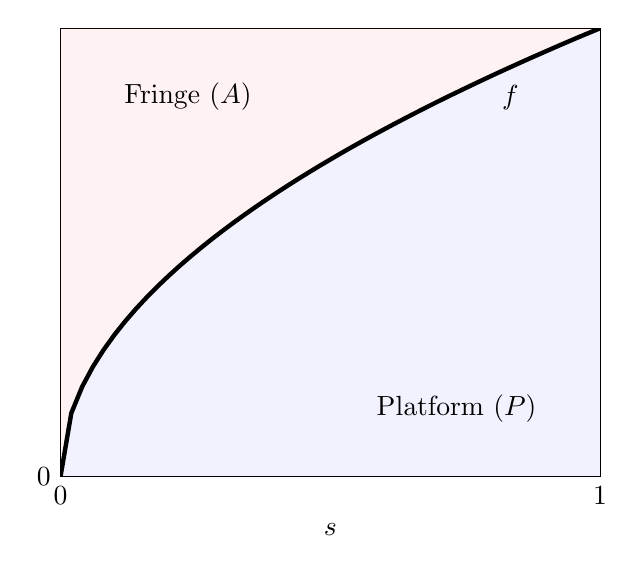
\begin{tikzpicture}
        \begin{axis}[xmin=0, xmax=1, ymin=0, ymax=1, samples at={0, 0.02, ..., 0.98, 1},
                xtick={0, 1}, ytick={0}, xlabel={$s$}]
            \addplot[name path=f, ultra thick] {x^0.5};
            \node[anchor=north west] at (axis cs: .8, .8^0.5) {$f$};
            \path[name path=bottom] (axis cs:0,0) -- (axis cs:1,0);
            \path[name path=top] (axis cs:0,1) -- (axis cs:1,1);

            \addplot [fill=blue, fill opacity=0.05] fill between [of=f and bottom];
            \addplot [fill=red, fill opacity=0.05] fill between [of=f and top];

            \node[anchor=north west] at (axis cs: .1, .9) {Fringe ($A$)};
            \node[anchor=south east] at (axis cs: .9, .1) {Platform ($P$)};
        \end{axis}
    \end{tikzpicture}
\end{figure}

Finally, the following corollary implies that, even though the individual share of each $A_i$ vanishes as their number goes to infinity, their total value still converges to a positive value.
\begin{corollary}
    \label{cor:fringe_value_2}
    $\varphi_P^\infty < f(1)$ and $\varphi_A^\infty > 0$ for any $f$ that is not constant.
\end{corollary}


\subsection{Weighted Shapley-values}

While the values of oceanic games (i.e. the limits of the Shapley values of their finite approximations in finite games) are well known in the relevant literature, there are no results about the limits of the weighted (Shapley) values.
While providing very general results in the form of \textcite[]{fogelman1980asymptotic} is outside the scope of the paper\footnote{
    They show that the (within some constraints) any discretization of an oceanic game converges to the same value.
} the results in this section still provide some new insights into weighted values of oceanic games.
In particular, I show that the weighted value of a game with one large and many small players converges to a rather simple and intuitive expression, if the size of the small players go to zero at the same rate.

Imagine a general non-cooperative game $(N, v)$ with $N = \{1, \dots, n\}$.
Assume that, in addition to the value function $v : 2^n \to \mathbb{R}$, the game is also endowed with a weight system $\lambda \in \mathbb{R}^n$.
These weights can be thought of as measures of innate bargaining power \parencite{shapley1953additive}, not reflected in the value function.
Further support for this interpretation can be found in \textcite{hart1996bargaining}, demonstrating that in a certain alternating offer bargaining game, weights are related to the probability of each player making the offer.\footnote{
    For example, only one player having a positive value corresponds to them making take it or leave it offers.
}

For my purposes, it is sufficient to deal with the case of simple weights. I.e., assume that there is at most one player with zero weight.
For my main result, I make use of the fact that weighted Shapley values can be calculated by weighting the permutations by the probabilities arising from the following sequential ordering procedure \parencite{kalai1987weighted}.
Start with the set of all players.
Let the probability of player $i$ being the last amongst the set of remaining players $R$ be $\lambda_i / \sum_{j \in R} \lambda_j$.
Continue until all players are exhausted.
This yields a well-defined probability for each permutation of players.

Consider the game described in the previous section, and let the weights of players of type $A$ and $P$ be 1 and $\lambda$, respectively.
Let $X_n$ be a random variable representing the number of players before $P$ when players are ordered according to the above procedure.
Then, the probability of player $P$ having at most $k$ players of type $A$ before themselves is simply
\begin{align*}
    \Pr(X_n \leq k) = \prod_{j=k+1}^n \frac{j}{j + \lambda} .
\end{align*}
The following lemma establishes the continuous analogue of this statement.
\begin{lemma}
    \label{lem:entry_distr}
     As $n \to \infty$, $X_n \xrightarrow[]{\mathrm{d}} X$ with the cdf $G_X(t) = \lambda^t$.
     Consequently, the corresponding probability density function is $g(t) = \lambda t^{\lambda - 1}$.
\end{lemma}

The main proposition of this section shows that the weighted Shapley-value of player $i$ can be expressed as the expected marginal contribution of that player where the permutations are weighted according to the previous distribution.
\begin{proposition}
    \label{prop:one_sided_weighted}
    Let $f(t)$ be continuous on $[0, 1]$. Then
    \begin{align*}
        \varphi_P(\lambda, \infty) = \int_0^1 g(t) f(t) \dt
    \end{align*}
    where $g(t) = \lambda t^{\lambda - 1}$.
\end{proposition}

\begin{figure}[ht]
    \centering
    \begin{subfigure}[b]{0.45\textwidth}
        \centering
        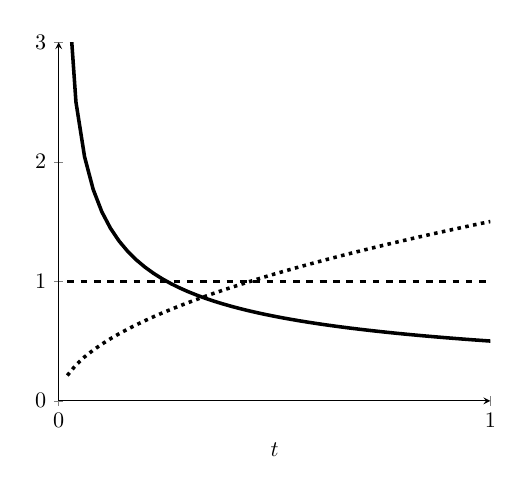
\begin{tikzpicture}[scale=0.8]
            \begin{axis}[xmin=0, xmax=1, ymin=0, ymax=3, samples at={0.02, 0.04, ..., 0.98, 1},
                xtick={0, 1}, ytick={0, 1, 2, 3}, axis lines=left, xlabel={$t$}, legend pos=south east]
                \addplot[ultra thick] {0.5 * x ^ (-0.5)};
                \addplot[ultra thick, dashed] {1};
                \addplot[ultra thick, dotted] {1.5 * x ^ (0.5)};
            \end{axis}
        \end{tikzpicture}
        \caption{$g(t)$}
    \end{subfigure}
    \begin{subfigure}[b]{0.45\textwidth}
        \centering
        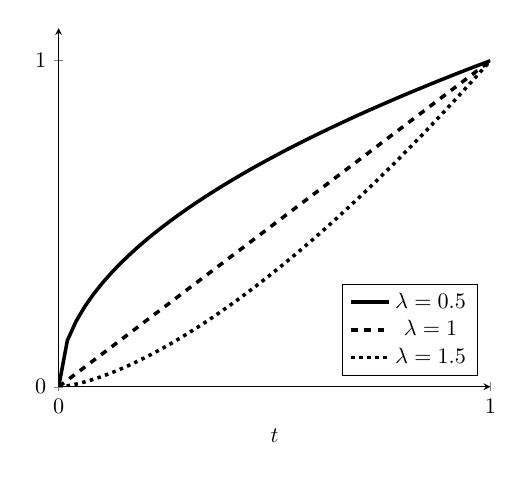
\begin{tikzpicture}[scale=0.8]
            \begin{axis}[xmin=0, xmax=1, ymin=0, ymax=1.1, samples at={0, 0.02, ..., 0.98, 1},
                xtick={0, 1}, ytick={0, 1}, axis lines=left, xlabel={$t$}, legend pos=south east]
                \addplot[ultra thick] {x ^ (0.5)};
                \addplot[ultra thick, dashed] {x};
                \addplot[ultra thick, dotted] {x ^ (1.5)};
                \legend{$\lambda = 0.5$, $\lambda = 1$, $\lambda = 1.5$}
            \end{axis}
        \end{tikzpicture}
        \caption{$\int_0^t g(s) \ds$}
    \end{subfigure}
    \caption{Illustration of the weighting function for various values of $\lambda$ in the weighted Shapley-value.}
    \label{fig:weigh_function}
\end{figure}

Finally, the following corollaries support the interpretation of weights as bargaining power, as a higher weight corresponds to a higher Shapley-value in this game.\footnote{
    This would not necessarily have to be the case, as demonstrated by \textcite{owen1968communications}.
}
Furthermore, the limit of the weighted value of $P$, as their weight goes to zero (infinity) is precisely the payoffs $P$ would achieve if $P$ were making (facing) take-it-or-leave-it offers.

\begin{corollary}
    \label{cor:platform_value_weighted}
    $\varphi_P(\lambda, \infty)$ is increasing in $\lambda$ unless $f$ is constant.
\end{corollary}

\begin{corollary}
    \label{cor:paltform_value_weighted_2}
    If the weight of player $P$ goes to infinity (zero), its weighted Shapley value converges to $f(1)$ ($f(0)$).
\end{corollary}

\subsection{Multiple platforms}

Imagine that, instead of just one, there are $m$ players of type $P$, and they are perfect substitutes of each other.
That is, the fringe players still need a platform to achieve any value, but it does not matter which or how many platforms are available for them.
Formally, the value function for coalition $S$ is the following:
\begin{align*}
    v(S) = \begin{cases}
        0                              & \text{if } n_P(S) = 0 \\
        f\left(\frac{n_A(S)}{n}\right) & \text{otherwise}.
    \end{cases}
\end{align*}

Let us start by establishing monotonicity for this version of the model, too.
\begin{proposition}
    The game is monotone if $f$ is increasing and $f(0) \geq 0$.
\end{proposition}
% \textcolor{red}{Note: I have to think more about how to describe this situation in the language of cooperative game theory. The issue is that, for example, the value of $\{P_1, A_1\}$ depends on whether $\{P_2, A_2\}$ also decides to form a coalition and enter the market.}

As before, the main proposition in this section provides us with an expression of the limit of the value for this variant of the game.
\begin{proposition}
    \label{prop:multiple_platforms}
    The limit of the Shapley-value (as $n \to \infty$) of each player of type $P$ is
    \begin{align*}
        \varphi_{P_i}^{\infty, m} = \int_0^1 (1-t) ^ {m-1} f(t) \dt .
    \end{align*}
\end{proposition}

\begin{figure}[ht]
    \centering
    \begin{subfigure}[b]{0.45\textwidth}
        \centering
        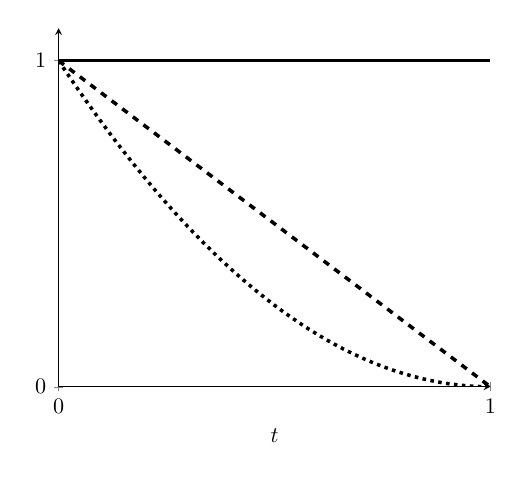
\begin{tikzpicture}[scale=0.8]
            \begin{axis}[xmin=0, xmax=1, ymin=0, ymax=1.1, samples at={0, 0.02, 0.04, ..., 0.98, 1},
                xtick={0, 1}, ytick={0, 1}, axis lines=left, xlabel={$t$}, legend pos=north west]
                \addplot[ultra thick] {1};
                \addplot[ultra thick, dashed] {1-x};
                \addplot[ultra thick, dotted] {(1-x)^2};
            \end{axis}
        \end{tikzpicture}
        \caption{$(1 - t) ^ {m - 1}$}
    \end{subfigure}
    \begin{subfigure}[b]{0.45\textwidth}
        \centering
        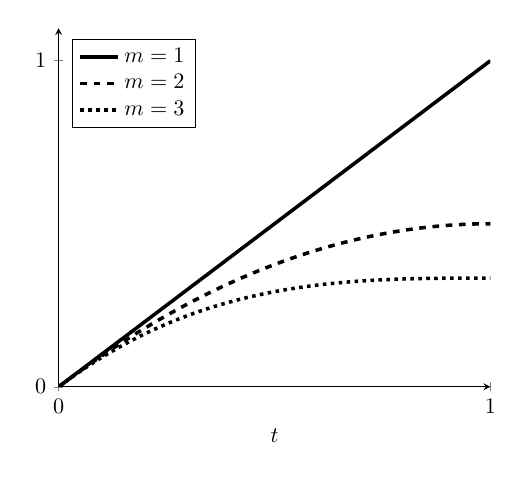
\begin{tikzpicture}[scale=0.8]
            \begin{axis}[xmin=0, xmax=1, ymin=0, ymax=1.1, samples at={0, 0.02, ..., 0.98, 1},
                xtick={0, 1}, ytick={0, 1}, axis lines=left, xlabel={$t$}, legend pos=north west]
                \addplot[ultra thick] {x};
                \addplot[ultra thick, dashed] {x - x^2/2};
                \addplot[ultra thick, dotted] {x - x^2 + x^3/3};
                \legend{$m = 1$, $m = 2$, $m = 3$}
            \end{axis}
        \end{tikzpicture}
        \caption{$\int_0^t (1 - s) ^ {m - 1} \ds$}
    \end{subfigure}
    \caption{Illustration of the weighting function for various values of $m$ in the multiple platform case.}
    \label{fig:multiple_platforms}
\end{figure}

As with proposition \ref{prop:one_sided}, this result also has a probabilistic interpretation, and could have been obtained directly using the axiomatic approach.
Let the location of the $m$ atoms be $t_1, \dots, t_m$, distributed independently and uniformly on the unit cube.
The expected marginal contribution of $t_i$ is only positive whenever it is the first amongst the major players.
That is, for any $t_i$, the probability if $P_i$ being the first is related to the cdf of the first order statistic from $n-1$ independent uniform distributions: $1 - (1-t)^{m-1}$.

\begin{corollary}
    \label{cor:multiple_platforms}
    The per-unit Shapley-value of the fringe is
    \begin{align*}
        \varphi_A(k, \infty) = 1 - m\int_0^1 (1-t) ^ {m-1} f(t) \dt = \int_0^1 [1 - (1-t)^m] f'(t) \dt .
    \end{align*}
\end{corollary}

The following corollary again demonstrates that the predicted outcomes confirm intuitions.
As the major players become more and more substitutable, the portion of the surplus they can capture decreases, and the aggregated value of the fringe increases.

\begin{corollary}
    \label{cor:multiple_platforms_2}
    Let $\varphi_{P}^{\infty, m} = m\varphi_{P_i}^{\infty, m}$ denote the aggregated values of players of type $P$. $\varphi_{P}^{\infty, m}$ is decreasing in $m$ and $\varphi_{A}^{\infty, m}$ is increasing in $m$ unless $f$ is constant.
\end{corollary}

\section{Many-sided case}

Now imagine that, in addition to player $P$, there are $L$ types of $n$ smaller players: $\{A^l_1, \dots, A^l_n\}$ where $1 \leq l \leq L$.
As before, $P$ is necessary for any coalition to have a positive value, and the small players are identical within their groups.
I.e., the set of players and the characteristic function of the game are the following: $N = \{P, A^1_1, \dots, A^1_n, \dots, A^L_1, \dots, A^L_n\}$ and
\begin{align*}
    v(S) = \begin{cases}
        0                                                & \text{if } P \notin S \\
        f\left(\frac{n_{A_1}(S)}{n}, \dots, \frac{n_{A_L}(S)}{n}\right) & \text{otherwise}.
    \end{cases}
\end{align*}
A prominent interpretation of the two-sided version this model would be a platform marketplace with a set of sellers and a set of buyers, where all three sides possess some amount of bargaining power.
However, player $P$ does not have to be in the ``middle'' of the transactions for this framework to be applicable.
For example, it also captures the situation of a single upstream producer, a large number of downstream firms, and a similarly large number of customers, as long as both the customers and the downstream firms can participate in the bargaining process.
A setting where these assumptions might be plausible is, for example, the new car market with a car producer, a number of independent dealerships, and customers who might engage in negotiation.

Let us follow the pattern from the previous sections.
Start by characterizing conditions for superadditivity to support the bargaining interpretation.
\begin{proposition}
    The game $(N, v)$ is monotone and superadditive if and only if $f$ is increasing in all of its arguments.
\end{proposition}

Next, let us obtain formulas for the values of the three groups of players.
It turns out that the limits of the Shapley-values (as $n \to \infty$) are still analytically tractable and they also have neat interpretations.
For ease of notation, let us define the following function:

\begin{proposition}
    Let $f$ be continuous everywhere on $[0, 1]^L$.
    Then,
    \begin{align*}
        \varphi_P^\infty & = \int_0^1 f(t, \dots, t) \dt                                 \\
        \varphi_{A_l}^\infty & = \int_0^1 t \partial_l f(t, \dots, t) \dt.
    \end{align*}
\end{proposition}

As the previous proposition shows, the value of each kind of player depends on their expected marginal contribution, i.e. the partial derivatives of $f$.
Consequently, the value of the grand coalition can be decomposed into the Shapley-values of its members signifying their expected marginal contributions in the following way:
\begin{align*}
    f(1, \dots, 1) = \underbrace{\int_0^1 f(t, \dots, t) \dt}_{\text{ player } P} + \sum_{l=1}^L \underbrace{\int_0^1 t \partial_l f(t, \dots, t) \dt}_{\text{players } A_l}.
\end{align*}

One surprising element of the result is that one only has to integrate over the diagonal of the support  of $f$, and the value does not depend on the marginal contributions in the case of an unequal measure of $A$ and $B$ types.
The intuition for that relies on a law-of-large-numbers-type reasoning.
If the number of fringe players is large, then it is very unlikely that, after a random ordering, their proportion in any interval will be too different.
Consequently, when taking the expectation over all orderings, ones with vary unequal numbers of the two types will have little impact on it.


\subsection{Multiple platforms}

The many-sided case can also simply be extended to incorporate multiple platforms instead of just one.
As before, assume that there are $k$ players of type $P$ which are perfect substitutes of each other:
\begin{align*}
    v(S) = \begin{cases}
        0                                                & \text{if } P_i \notin S \; \forall \, i = 1, \dots, k \\
        f\left(\frac{n_{A_1}(S)}{n}, \dots, \frac{n_{A_L}(S)}{n}\right) & \text{otherwise}.
    \end{cases}
\end{align*}

It can be shown that the values of each type of player are rather similar to the one-platform case.
\begin{proposition}
    The unit Shapley-values of the various types of players are
    \begin{align*}
        \varphi_{P_i}(k, \infty) & = \int_0^1 (1-t)^{k-1} f(t, \dots, t) \dt                                 \\
        \varphi_{A_l}(k, \infty)     & = \int_0^1 [1 - (1-t)^k] \partial_l f(t, \dots, t) \dt.
    \end{align*}
\end{proposition}

Similarly, as the next corollary demonstrates, the combined value of platforms is still decreasing in their number.
\begin{corollary}
    Let $\varphi_{P}(k, \infty) = k\varphi_{P_i}(k, \infty)$ denote the aggregated Shapley-values of players of type $P$.
    Then $\varphi_{P}(k, \infty)$ is decreasing in $k$ and $\varphi_{A_l}(k, \infty)$ are increasing in $k$ unless $f$ is constant.
\end{corollary}


\section{Example Application}

This section demonstrates the proposed cooperative approach via a model of a vertical market.
Note, that this is not a full-fledged model, and many factors are exogenous.
However, it is sufficient to illustrate the advantages of the framework presented in this paper: most notably, its analytical tractability and that it captures what intuitively feels like bargaining power.

Consider a market in the vein of \textcite{hart1990property}, but with a finite number of upstream and a continuum of downstream firms.
Furthermore, let us model production and sales in a reduced form, without going into the micro-foundations of the profit functions.
Finally, let us assume that profits are shared according to players' Shapley-values.

In the rest of this section, I will examine the effect of various market structures on the profit distribution.
I start by looking at the case of a single upstream producer, with no direct acces to the downstream market.
I then contrast this with two scenarios in which the upstream producer acquires a way to directly sell to the final consumers: either by vertical integration (merging with some share of the downstream firms), or by creating a completely new, downstream division within itself.

As this model is only supposed to be an illustration, I will focus on simplicity rather than realism.
Furthermore, I will not endogenize certain choices, such as entry, or the actual merger decisions.
Nevertheless, some of the results are suggestive of what might happen in an applied, more fully specified model.


\subsection{Benchmark case}

Let us start by looking at the simplest case: one upstream producer, no direct access to the downstream market.
Assume that without the upstream producer, the downstream firms cannot produce anything, and thus total industry profits are zero.
On the other hand, if the upstream producer and $t$ fraction of the downstream firms create an agreement, then total industry profits are given by the function $f(t)$.\footnote{
    This reduced-form profit function can be given microfoundations in many ways.
    For an example, see \textcite{stancsics2023hybrid}.
}
Furthermore, the following assumption guarantees ensures that the game is superadditive, therefore it actually makes sense to have every downstream firm in the coalition.\footnote{
    TODO: elaborate on what this assumption entails.
}
\begin{assumption}
    Let us assume that $f$ is continuous and increasing in $t$.
\end{assumption}

As noted before, profits are distributed according to players' Shapley values.
Consequently, it follows from \cref{prop:one_sided} that the profits of the upstream producer and the downstream mass of firms are
\begin{align*}
    \pi_P^b & = \int_0^1 f(t) \dt, \\
    \pi_A^b & = f(1) - \int_0^1 f(t) \dt,
\end{align*}
respectively.


\subsection{Vertical integration}

Let us now consider the case in which the upstream producer merges with some fraction $\alpha$ of the downstream firms.
The total profits are the same as before, namely, $f(1)$.\footnote{
    TODO: do I need a footnote here?
}
However, the profit distribution is now different.
New shares can be calculated as follows:
\begin{align}
    \pi_{P}^m & = \frac{1}{1 - \alpha} \int_\alpha^1 f(t) \dt, \\
    \pi_{A}^m & = f(1) - \frac{1}{1 - \alpha} \int_\alpha^1 f(t) \dt .
\end{align}

Clearly, the upstream producer gets a larger share than before, while the remaining downstream firms capture a smaller share.
This is intuitive, as the upstream producer now depends on the remaining downstream sellers to a lesser extent.
However, it's worth examining whether this increase is large enough in the sense that the now hybrid upstream producer's profit is higher than the sum of its profit and $\alpha$ fraction of the downstream firms' profit from the benchmark case.
The participants only have an incentive to merge if this is the case.
It turns out that this depends on the shape of the profit function.\footnote{
    This way of modeling vertical integration assumes that the upstream firm's innate bargaining power is not affected by the merger.
    In the terms of some non-cooperative bargaining model, such as \textcite{hart1996bargaining}, it means that the non-acquired downstream firms get a higher probability of proposing allocations.
    It could be interesting to see how the results change when the upstream firm's also obtains the acquired downstream firms' innate bargaining power, and profits are distributed according to weighted Shapley values.
}

\begin{proposition}
    \label{prop:vertical_integration}
    If $f$ is concave (convex) on $[0, 1]$, then $\pi_P^m \geq \pi_P^b + \alpha \pi_A^b$ ($\pi_P^m \leq \pi_P^b + \alpha \pi_A^b$). 
\end{proposition}

\begin{figure}[ht]
    \centering
    \begin{subfigure}[b]{0.45\textwidth}
        \centering
        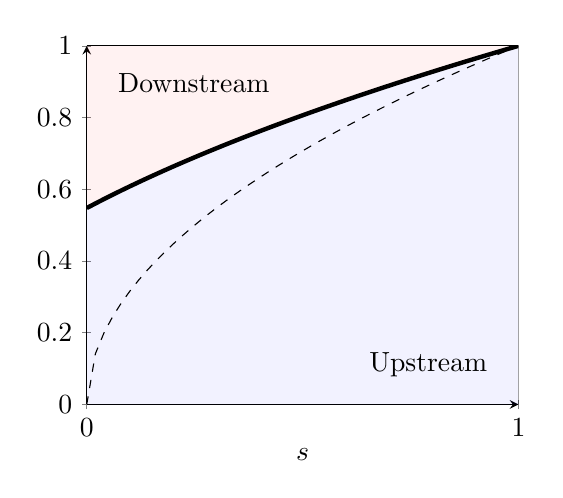
\begin{tikzpicture}[scale=0.8]
            \begin{axis}[xmin=0, xmax=1, ymin=0, ymax=1, samples at={0, 0.02, ..., 0.98, 1},
                xtick={0, 1}, 
                axis lines=left, xlabel={$s$}]
                \addplot[name path=f, dashed, black] {sqrt(x)};
                \addplot[name path=tildef, black, ultra thick] {sqrt(0.3+0.7*x)};
                \path[name path=bottom] (axis cs:0,0) -- (axis cs:1,0);
                \draw[name path=top] (axis cs:0,1) -- (axis cs:1,1);
                \draw[name path=right] (axis cs:1,0) -- (axis cs:1,1);
    
                \addplot [fill=blue, fill opacity=0.05] fill between [of=tildef and bottom];
                \addplot [fill=red, fill opacity=0.05] fill between [of=tildef and top];
    
                \node[anchor=north west] at (axis cs: .05, .95) {Downstream};
                \node[anchor=south east] at (axis cs: .95, .05) {Upstream};
            \end{axis}
        \end{tikzpicture}
        \caption{Concave case}
    \end{subfigure}
    \begin{subfigure}[b]{0.45\textwidth}
        \centering
        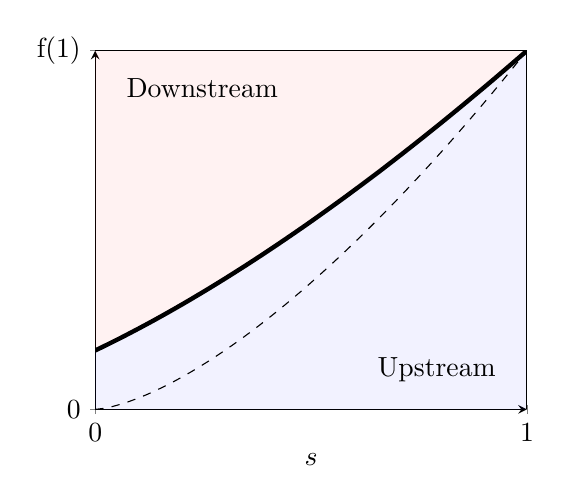
\begin{tikzpicture}[scale=0.8]
            \begin{axis}[xmin=0, xmax=1, ymin=0, ymax=1, samples at={0, 0.02, ..., 0.98, 1},
                xtick={0, 1}, ytick={0, 1}, yticklabels={0, f(1)},
                axis lines=left, xlabel={$s$}]
                \addplot[name path=f, dashed, black] {(x)^1.5};
                \addplot[name path=tildef, black, ultra thick] {(0.3+0.7*x)^1.5};
                \path[name path=bottom] (axis cs:0,0) -- (axis cs:1,0);
                \draw[name path=top] (axis cs:0,1) -- (axis cs:1,1);
                \draw[name path=right] (axis cs:1,0) -- (axis cs:1,1);
    
                \addplot [fill=blue, fill opacity=0.05] fill between [of=tildef and bottom];
                \addplot [fill=red, fill opacity=0.05] fill between [of=tildef and top];
    
                \node[anchor=north west] at (axis cs: .05, .95) {Downstream};
                \node[anchor=south east] at (axis cs: .95, .05) {Upstream};
            \end{axis}
        \end{tikzpicture}
        \caption{Convex case}
    \end{subfigure}
    \caption{Illustration of \cref{prop:vertical_integration}}
    \label{fig:vertical_intergration}
\end{figure}

The intuition is that when $f$ is concave, then obtaining some fraction of the firms lets it create a (comparatively) large share of the total possible profits by itself, and its bargaining position is considerably strengthened.
In comparison, when $f$ is convex, then the upstream producer still has a large need for the rest of the downstream firms, even when it acquires some of them.
The bottom line is that industries which are characterized by the downstream firms being relatively substitutable are more susceptible to consolidation.

\subsection{Upstream firm builds downstream capacity}

Now let us consider another way of getting direct downstream access: instead of acquiring some of the existing downstream firms, the upstream producer creates new downstream capacity from scratch.
In contrast to the previous case, the total size of the pie also changes.
Let's assume that the upstream firm's downstream capacity is equal to that of $\alpha$ measure of the downstream firms.
Then, the total profits when everyone agrees to participate is given by $f(1 + \alpha)$, which is larger than $f(1)$ before.

As before, let us examine the distribution of the profits in this case as well:
\begin{align*}
    \pi_{P}^c & = \int_0^1 f(t + \alpha) \dt, \\
    \pi_{A}^c & = f(1 + \alpha) - \int_0^1 f(t + \alpha) \dt .
\end{align*}
Similarly to the vertical merger case, the now hybrid upstream producer's profits increase with the size of its downstream capacity.
However, it is not obvious how the downstream's profit changes.
The next proposition shows that it, again, depends on the shape of the profit function.
\begin{proposition}
    \label{prop:downstream_capacity}
    If $f$ is concave (convex) on $[0, 1+\alpha]$, then $\pi_A^m \geq \pi_A^b$ ($\pi_A^m \leq \pi_A^b$). 
\end{proposition}

\begin{figure}[ht]
    \centering
    \begin{subfigure}[b]{0.45\textwidth}
        \centering
        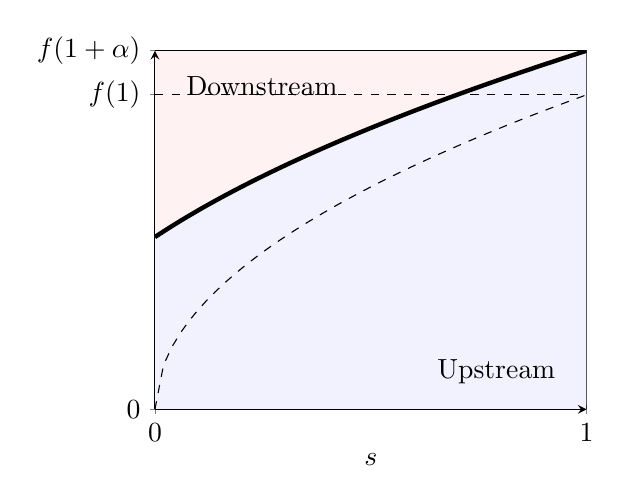
\begin{tikzpicture}[scale=0.8]
            \begin{axis}[xmin=0, xmax=1, ymin=0, ymax=1.14, samples at={0, 0.02, ..., 0.98, 1},
                xtick={0, 1}, ytick={0, 1, 1.14}, yticklabels={$0$, $f(1)$, $f(1 + \alpha)$},
                axis lines=left, xlabel={$s$}]
                \addplot[name path=f, dashed, black] {sqrt(x)};
                \addplot[name path=tildef, black, ultra thick] {sqrt(0.3+x)};
                \draw[dashed] (axis cs:0,1) -- (axis cs:1,1);
                \path[name path=bottom] (axis cs:0,0) -- (axis cs:1,0);
                \draw[name path=top] (axis cs:0,1.14) -- (axis cs:1,1.14);
                \draw[name path=right] (axis cs:1,0) -- (axis cs:1,1.14);
    
                \addplot [fill=blue, fill opacity=0.05] fill between [of=tildef and bottom];
                \addplot [fill=red, fill opacity=0.05] fill between [of=tildef and top];
    
                \node[anchor=north west] at (axis cs: .05, 1.09) {Downstream};
                \node[anchor=south east] at (axis cs: .95, .05) {Upstream};
            \end{axis}
        \end{tikzpicture}
        \caption{Concave case}
    \end{subfigure}
    \begin{subfigure}[b]{0.45\textwidth}
        \centering
        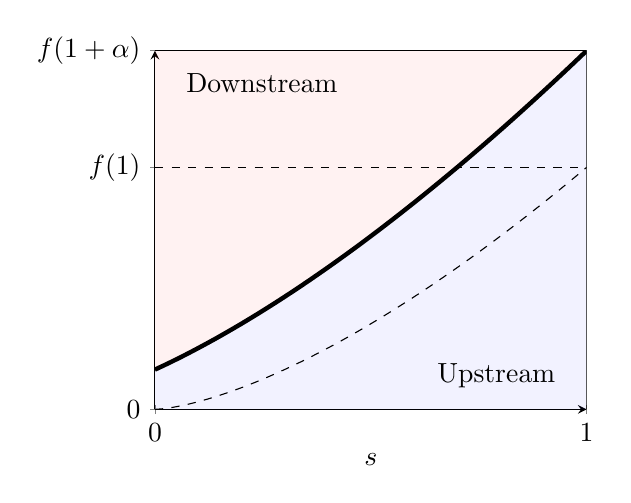
\begin{tikzpicture}[scale=0.8]
            \begin{axis}[xmin=0, xmax=1, ymin=0, ymax=1.482, samples at={0, 0.02, ..., 0.98, 1},
                xtick={0, 1}, ytick={0, 1, 1.482}, yticklabels={$0$, $f(1)$, $f(1 + \alpha)$},
                axis lines=left, xlabel={$s$}]
                \addplot[name path=f, dashed, black] {(x)^1.5};
                \addplot[name path=tildef, black, ultra thick] {(0.3+x)^1.5};
                \draw[dashed] (axis cs:0,1) -- (axis cs:1,1);
                \path[name path=bottom] (axis cs:0,0) -- (axis cs:1,0);
                \draw[name path=top] (axis cs:0,1.482) -- (axis cs:1,1.482);
                \draw[name path=right] (axis cs:1,0) -- (axis cs:1,1.482);
    
                \addplot [fill=blue, fill opacity=0.05] fill between [of=tildef and bottom];
                \addplot [fill=red, fill opacity=0.05] fill between [of=tildef and top];
    
                \node[anchor=north west] at (axis cs: .05, 1.43) {Downstream};
                \node[anchor=south east] at (axis cs: .95, .05) {Upstream};
            \end{axis}
        \end{tikzpicture}
        \caption{Convex case}
    \end{subfigure}
    \caption{Illustration of \cref{prop:downstream_capacity}}
    \label{fig:upstream_capacity}
\end{figure}

The results are similar to the previous case.
When the downstream firms are more substitutable, the upstream firms' newly created capacity strongly reduces their bargaining power, and even though the total size of the pie increases, the downstream firms' share decreases not only in relative terms, but also in absolute terms.
In a model with endogenous entry and exit on the part of the downstream firms, this would most likely lead to a reduction in their number.
The implication then also resembles the one in the vertical merger case: industries when downstream firms are easily substitutable should be strongly scrutinized when an upstream firm seeks to build its own downstream capacity.


\section{Conclusions}

This paper proposed a new framework to think about the profit allocation in situations concerning a few large and a continuum of smaller players.
The results are especially relevant for upstream-downstream situations, platform settings, and two-sided markets.
The outcomes of the Shapley-value-based gain sharing rule generally concur with intuitive expectations, and the resulting formulas are more tractable than most explicit non-cooperative approaches.

The illustrative model also highlights the strengths of this approach.
Despite its simplicity, it highlights that the effects of vertical integration strongly depends on the substitutability of the downstream firms.
In a time when upstream firms and platforms are increasingly seeking to sell directly to the consumers\footnote{
    As some recent examples, consider the recent acquisition of Whole Foods by Amazon, Microsoft's ongoing efforts to buy Activision/Blizzard (a major video game publisher), or Tesla's or BMW's plans to sell cars directly without the help of dealerships.
}
, such results can be important for competition authorities.

There is a variety of ways through which this paper could be expanded or built upon.
On the theoretical side, a number of the assumptions, such as fringe agents achieving a zero payoff without the platform, could be relaxed,
Besides this, the convergence result for the weighted values could be strengthened if one could manage to show that any sequence along ever more refined partitions of the atomic players converges to the same limit \parencite[à la][]{fogelman1980asymptotic}.

A slightly different direction would be to consider other solution concepts from cooperative game theory in this specific setting.
One obvious candidate is the nucleolus, which shares many of the useful properties of the Shapley-value (it always exists and is unique).
Furthermore, it also has connections to bargaining theory due to it being contained in the core when the latter exists.

The possibilities for practical applications are no less interesting.
The proposed profit sharing framework could be embedded in a more applied model of some real-life setting.
For a step in this direction, see \textcite{stancsics2023hybrid}.

Finally, with time, the cooperative approach to profit distribution could become an almost drop-in alternative of the more usual, but in some sense more extreme assumptions about the bargaining process widely used in industrial organization models.


\appendix

\printbibliography

\section{Miscellaneous lemmas}

\begin{lemma}
    \label{lemma:log_convergence}
    Let 
    \begin{align*}
        \Delta_n(s) &= \frac{\log(s + 1/n) - \log(\lambda)}{n}, \\
        \Delta(s) &= \frac{1}{s}.
    \end{align*}
    Then $\Delta_n \xrightarrow[]{\mathrm{u}} \Delta$ uniformly on $[t, 1]$ for any $t > 0, \lambda > 0$.
\end{lemma}
\begin{proof}[Proof of Lemma \ref{lemma:log_convergence}]
    First, note that $\Delta_n$ and $\Delta$ are all continuous functions.
    Then, following the standard proof for $\frac{\mathrm{d}}{\mathrm{d}s}log(s) = \frac{1}{s}$ rewrite $\Delta_n(s)$ as
    \begin{align*}
        \Delta_n(s) &= \frac{\log(s + 1/n) - \log(\lambda)}{n} \\
        &= \log \left( 1 + \frac{1}{sn} \right) ^ n .
    \end{align*}
    It is well known that $\left( 1 + \frac{1}{sn} \right) ^ n$ is monotone increasing in $n$ and converges to $\exp (1/s)$.
    Therefore, the pointwise convergence of $\Delta_n(s) \to \Delta(s)$ is also monotone.

    Finally, by Dini's theorem, the monotone pointwise convergence of a sequence of continuous functions to a continuous function on a compact set implies uniform convergence on that set.
\end{proof}

\begin{lemma}
    \label{lemma:integral_convergence}
    Let $f_n, f: [a, b] -> \mathbb{R}$ be Riemann-integrable functions with $f_n \xrightarrow[]{\mathrm{u}} f$ uniformly.
    Then,
    \begin{align*}
        \lim_{n \to \infty} \frac{b-a}{n} \sum_{k=1}^n f_n \left( a + \frac{b-a}{n} \right) = \int_0^1 f(t) \dt.
    \end{align*}
\end{lemma}
\begin{proof}[Proof of Lemma \ref{lemma:integral_convergence}]
    \begin{align*}
        &\lim_{n \to \infty} \frac{b-a}{n} \sum_{k=1}^n f_n \left( a + \frac{b-a}{n} \right) \\
        &= \lim_{n \to \infty} \frac{b-a}{n} \left[ \sum_{k=1}^n f \left( a + \frac{b-a}{n} \right) + \sum_{k=1}^n \left( f_n \left( a + \frac{b-a}{n} \right) - f \left( a + \frac{b-a}{n} \right) \right) \right] \\
        &= \int_a^b f(t) \dt + \lim_{n \to \infty} \frac{b-a}{n}\sum_{k=1}^n \left( f_n \left( a + \frac{b-a}{n} \right) - f \left( a + \frac{b-a}{n} \right) \right) \\
        &\leq \int_a^b f(t) \dt + \lim_{n \to \infty} \frac{b-a}{n}\sum_{k=1}^n \left| f_n \left( a + \frac{b-a}{n} \right) - f \left( a + \frac{b-a}{n} \right) \right| \\
        &\leq \int_a^b f(t) \dt + \lim_{n \to \infty} \frac{b-a}{n}\sum_{k=1}^n \sup_{t \in [a, b]} \left| f_n(t) - f(t) \right| \\
        &= \int_a^b f(t) \dt + (b-a) \underbrace{\lim_{n \to \infty} \sup_{t \in [a, b]} \left| f_n(t) - f(t) \right|}_{=0 \text{ due to uniform convergence}} \\
        &= \int_a^b f(t) \dt
    \end{align*}
\end{proof}


\section{Proofs of propositions and lemmas in the main text}

\begin{proof}[Proof of Proposition \ref{prop:monotone}]
    Monotonicity is evident.
    For superadditivity, note that for any coalitions $S_1, s_2$ such that $S_1 \cap s_2 = \emptyset$, $P \notin S_1$ or $P \notin s_2$.
    WLOG assume it is the latter, therefore $v(S_2) = 0$.
    As a result, $v(S_1) + v(S_2) = v(S_1) \leq v(S_1 \cup S_2)$ holds if and only if $(N, v)$ is monotone.
\end{proof}

\begin{proof}[Proof of Proposition \ref{prop:one_sided}]
    Let $R$ denote a permutation of the set of players ($N$).
    Additionally, let us denote the players preceding $i$ by $\mathcal{P}_i^R$.
    The value of player $P$ is their expected marginal contribution averaged over all permutations of $N$:
    \begin{align*}
        \varphi_P^n = \frac{1}{(n+1)!} \sum_R v(\mathcal{P}_P^R \cup \{i\}) - v(\mathcal{P}_P^R)
    \end{align*}
    First, note that $v(\mathcal{P}_P^R) = 0$ for any permutation, as no coalition can achieve a positive value without player $P$.
    Furthermore, using the fact that all agents of type $A$ are identical implies that $v(\mathcal{P}_P^R \cup \{i\})$ only depends on the number of agents in the coalition.
    More precisely, 
    \begin{align*}
        v(\mathcal{P}_P^R \cup \{i\}) = f(n_A(\mathcal{P}_P^R \cup \{i\}) / n) = f(|\mathcal{P}_P^R| / n).
    \end{align*}
    Finally, the set of permutations in which $k$ number of players precede $P$ is independent of $n$, i.e.
    \begin{align*}
        \{R \mid |\mathcal{P}_P^R| = k\} = n! \quad \forall\, k.
    \end{align*}
    Putting all the above together, the value of player $P$ can be expressed as
    \begin{align*}
        \varphi_P^n &= \frac{1}{(n+1)!} \sum_{k=0}^n n! f(k / n) \\
        &= \frac{1}{n+1} \sum_{k=0}^n f(k / n) \\
        &= \frac{n}{n+1} \underbrace{\frac{1}{n} \sum_{k=0}^{n-1} f(k / n)}_{=S_n} + \frac{1}{n+1} f(1).
    \end{align*}
    $S_n$ are just the left Riemann-sums of function $f$ on the interval $[0, 1]$.
    Therefore, if $f$ is continuous (and thus Riemann-integrable), then $S_n \to \int_0^1 f(t)$, and thus
    \begin{align*}
        \lim_{n \to \infty} \varphi_P^n &= \lim_{n \to \infty} \frac{1}{n+1} \sum_{k=1}^n f(k / n) \\
        &= \lim_{n \to \infty}\underbrace{\frac{n}{n+1}}_{\to 1} \frac{1}{n} \sum_{k=0}^{n-1} f(k / n) + \underbrace{\frac{1}{n+1} f(1)}_{\to 0} \\
        &= \int_0^1 f(t) \dt .
    \end{align*}
\end{proof}

\begin{proof}[Proof of Corollary \ref{cor:fringe_value}]
    The first equality comes from the efficiency of the Shapley-value.
    The values of all players sum up to $f(1)$ for all $n \in \mathbb{N}$, therefore
    \begin{align*}
        \lim_{n \to \infty} \sum_{i=1}^n \varphi_{A_i}^n = \lim_{n \to \infty} (1 - \varphi_P^n ) = 1 - \int_0^1 f(t).
    \end{align*}
    The second can be obtained by integration by parts:
    \begin{align*}
        \int_0^1 t f'(t) \dt = tf(t) \mid_0^1 - \int_0^1 f(t) \dt = f(1) - \int_0^1 f(t) \dt
    \end{align*}
\end{proof}

\begin{proof}[Proof of Lemma \ref{lem:entry_distr}] %\textcolor{red}{(Might have to fix sum indices)} \\
    The probability of $P$ having at most fraction $t$ of the other players before itself is
    \begin{align*}
        \Pr(X_n \leq nt) &= \Pr(X_n \leq nt ) \\
        &= \prod_{j = nt + 1}^n \frac{j}{j + \lambda} \\
        &= \exp \Bigg( \underbrace{\sum_{j = nt + 1}^n \log(j) - \log(j+\lambda)}_{\equiv S_n} \Bigg).
    \end{align*}
    Taking limits,
    \begin{align*}
        \lim_{n \to \infty} S_n &= \lim_{n \to \infty} \sum_{j = nt + 1}^n \log(j) - \log(j+\lambda) \\
        &= \lim_{n \to \infty} \sum_{i = 1}^{n - nt} \log(nt + i) - \log(nt + i + \lambda) \\
        &= \lim_{n \to \infty} \frac{1}{n - nt} \sum_{i = 1}^{n - nt} \frac{\log \left( t + \frac{i}{n - nt} \right) - \log \left( t + \frac{i}{n - nt} + \frac{\lambda}{n - nt} \right)}{1 / (n - nt)}
    \end{align*}
    Let
    \begin{align*}
        \Delta_n(s) = \frac{\log \left( s \right) - \log \left( s + \frac{\lambda}{n - nt} \right)}{1 / (n - nt)}
    \end{align*}
    By lemma \ref{lemma:log_convergence}, 
    \begin{align*}
        \Delta_n \xrightarrow[]{\mathrm{u}} \lambda \frac{\mathrm{d}}{\mathrm{d}s}log(s) = -\frac{\lambda}{s}
    \end{align*}
    on the compact interval $[t, 1]$ for any $t > 0$ ($\xrightarrow[]{\mathrm{u}}$ denotes uniform convergence).
    
    Then, by lemma \ref{lemma:integral_convergence}, we have that
    \begin{align*}
        \lim_{n \to \infty} S_n &= \lim_{n \to \infty} \frac{1}{n-nt} \sum_{i=1}^{n-nt} \Delta_n \left( t + \frac{i}{n - nt} \right) \\
        &= \int_t^1 (\lim_{n \to \infty} \Delta_n)(s) \ds \\
        &= \int_t^1 \lim_{n \to \infty} -\frac{\lambda}{s} \ds \\
        &= \lambda \log{t}
    \end{align*}

    Substituting $\lim_{n \to \infty} S_n$ into the original equation yields
    \begin{align*}
        \lim \Pr \left( \frac{X_n}{n} \leq t \right) &= \exp \Bigg( \lim_{n \to \infty} \sum_{j = nt + 1}^n \log(j) - \log(j+\lambda) \Bigg) \\
        &= \exp(\lambda \log(t)) \\
        &= t^\lambda.
    \end{align*}

    For $t=0$, simply observe that %\textcolor{red}{Have to elaborate on this}
    \begin{align*}
        \lim_{n \to \infty} \prod_{j = 1}^n \frac{j}{j + \lambda} = 0 = 0^\lambda.
    \end{align*}
\end{proof}

\begin{proof}[Proof of Corollary \ref{cor:fringe_value_2}]
    If $f$ is monotone increasing, then $f(0) \leq \int_0^1 f(t) \dt \leq f(1)$.
    The inequalities become strict if $f$ is not constant on the whole interval.
\end{proof}

\begin{proof}[Proof of Proposition \ref{prop:one_sided_weighted}]
    The weighted value of player $P$ is its expected contribution across all permutations, with each permutation weighted by its probability of occurring.
    \begin{align*}
        \varphi_P^{n, \lambda} = \sum_R \Pr(R) [v(\mathcal{P}_P^R \cup \{i\}) - v(\mathcal{P}_P^R)]
    \end{align*}
    As before, using the fact that fringe players are identical, this can be rephrased as
    \begin{align*}
        \varphi_P^{n, \lambda} &= \sum_{k=0}^n \Pr(R) f(k/n) \\
        &= \E[f(X_n / n)]
    \end{align*}
    where $X_n$ is defined as above.
    $f$ is continuous, and therefore bounded on the compact set $[0, 1]$.
    As a consequence, $\frac{X_n}{n} \xrightarrow[]{\mathrm{d}} X$ implies $\E[f(X_n / n)] \to \E[f(X)]$, which in turn gives
    \begin{align*}
        \lim_{n \to \infty} \varphi_P^{n, \lambda} &= \lim_{n \to \infty} \E[f(X_n / n)] \\
        &= \E[f(X)] \\
        &= \int_0^1 f(t) \mathrm{d}G(t) \\
        &= \int_0^1 g(t)f(t) \dt
    \end{align*}
    where $G(t)$ and $g(t)$ are the cdf and pdf of X, respectively.
\end{proof}

\begin{proof}[Proof of Corollary \ref{cor:platform_value_weighted}]
    Let $X$ and $X'$ be random variables with cdfs $G_X = t^\lambda$ and $G_{X'}t^{\lambda'}$, respectively.
    For any $\lambda < \lambda'$, $t^\lambda > t^{\lambda'} \forall t \in [0, 1]$, meaning that $X'$ first-order stochastically dominates $X'$.
    As a result, for any monotonically increasing $f$,
    \begin{align*}
        \int_0^1 g_X(t)f(t) \dt = \E[f(X)] \leq \E[f(X')] = \int_0^1 g_{X'}(t)f(t)
    \end{align*}
    with strict inequality unless $f$ is constant almost everywhere.
    As $f$ is continuous, the latter is equivalent to $f$ being constant on the whole $[0, 1]$ interval.
\end{proof}

\begin{proof}[Proof of Corollary \ref{cor:paltform_value_weighted_2}]
    As $\lambda \to 0$, $X$ converges to the degenerate random variable $X_0$ for which $\Pr(X_0 = 0) = 1$.
    As a consequence, the expected value of $f(X)$ converges to $\E[f(X_0)] = f(0)$.
    $\lim_{\lambda \to \infty} \varphi^{\infty, \lambda}_P = f(1)$ can be shown along the same lines.
\end{proof}

\begin{proof}[Proof of Proposition \ref{prop:multiple_platforms}]
    \label{prop:one_sided_multiple}
    First, let us rewrite the expected marginal contribution of player $P_i$ in the following way:
    \begin{align*}
        \varphi_{P_i}^{n, m} &= \frac{1}{(n+m)!} \sum_R v(\mathcal{P}_{P_i}^R \cup \{i\}) - v(\mathcal{P}_{P_i}^R) \\
        &= \frac{1}{(n+m)!} \left[ \sum_{\{R | n_P(\mathcal{P}_{P_i}^R = 0)\}} \left[v(\mathcal{P}_{P_i}^R \cup \{i\}) - v(\mathcal{P}_{P_i}^R)\right] + \sum_{\{R | n_P(\mathcal{P}_{P_i}^R > 0)\}} \left[v(\mathcal{P}_{P_i}^R \cup \{i\}) - v(\mathcal{P}_{P_i}^R)\right] \right]
    \end{align*}
    Next, make use of the fact that the marginal contribution of a platform is zero if another platform is already present, and only depends on the number of fringe firms otherwise.
    \begin{align*}
        \varphi_{P_i}^{n, m} &= \frac{1}{(n+m)!} \sum_{\{R | n_P(\mathcal{P}_{P_i}^R = 0)\}} f (\mathcal{P}_{A}^R / n) \\
        &= \frac{1}{(n+m)!} \sum_{k=0}^n |\{R | n_A(\mathcal{P}^R_{P_i} = k) \text{ and } n_P(\mathcal{P}^R_{P_i} = 0)\}| f(k/n)
    \end{align*}
    Finally, notice that, while the permutations with $k$ fringe agents before $P_i$ does not depend on $k$, amongst those, the number of permutations with no platform before $P_i$ does depend on it.
    In particular,
    \begin{align*}
        |\{R | n_A(\mathcal{P}^R_{P_i} = k) \text{ and } n_P(\mathcal{P}^R_{P_i} = 0)\}| &= \frac{n!(n+m-k-1)!}{(n-k)!}
    \end{align*}
    and
    \begin{align*}
        \varphi_{P_i}^{n, m} &= \sum_{k=0}^n \frac{n!(n+m-k-1)!}{(n+m)!(n-k)!} f(k/n) \\
        &= \sum_{k=0}^n \frac{(n-k+1)(n-k+2) \dots (n-k+m-1)}{(n+1)(n+2) \dots (n+m)} f(k/n) \\
        &= \frac{1}{n+1}\sum_{k=0}^n \underbrace{\frac{(n(1-k/n)+1)(n(1-k/n)+2) \dots (n(1-k/n)+m-1)}{(n+2) \dots (n+m)} f(k/n)}_{S_n}
    \end{align*}
    For any $t = k/n \in [0, 1]$, 
    \begin{align*}
        S_n(t) \to (1-t)^{m-1}f(t) \equiv S(t).
    \end{align*}
    Furthermore, it is simple to verify that this convergence is uniform, and that $S_n$ and $S$ are all continuous functions.
    By Dini's theorem, the former properties imply that $S_n \xrightarrow[]{\mathrm{u}} S$ uniformly on $[0, 1]$.

    The conclusion of the proof is similar to that of proposition \ref{prop:one_sided}:
    \begin{align*}
        \lim_{n \to \infty} \varphi_{P_i}^{n, m} &= \lim_{n \to \infty} \underbrace{\frac{n}{n+1}}_{\to 1} \sum_{k=0}^{n-1} S_k(k/n) + \underbrace{\frac{1}{1+n}S(1)}_{\to 0} \\
        &= \lim_{n \to \infty} \sum_{k=0}^{n-1} S_k(k/n) \\
        &= \int_0^1 (1-t)^{m-1} f(t) \dt
    \end{align*}
    with the last equality supported by lemma \ref{lemma:integral_convergence}.
\end{proof}

\begin{proof}[Proof of Corollary \ref{cor:multiple_platforms}]
    The allocation is efficient for all $n \in \mathbb{N}$, therefore efficient in the limit, as well.
    The second equality can be obtained by integration by parts.
\end{proof}

\begin{proof}[Proof of Corollary \ref{cor:multiple_platforms_2}] (Assuming $f$ is continuously differentiable) %\textcolor{red}{(Assuming $f$ is continuously differentiable -- will have to relax this)}
    $f'(t)$ is non-negative, so $[1 - (1-t)^m] f'(t)$ is increasing in $m$ $\forall t \in [0, 1]$.
    As a consequence, $\varphi_A^{n, \infty}$ is also increasing in $m$ if $f'(t)$ is positive on some interval or, $f(t)$ is not constant.
    Conversely, $\varphi_{P}^{\infty, m} = 1 - \varphi_{A}^{\infty, m}$ is decreasing in $m$.
\end{proof}

\end{document}
